\chapter{ПРИЛОЖЕНИЕ Б}
\section{Дополнительные результаты тестирований}

\begin{figure}[h]
    \centering
    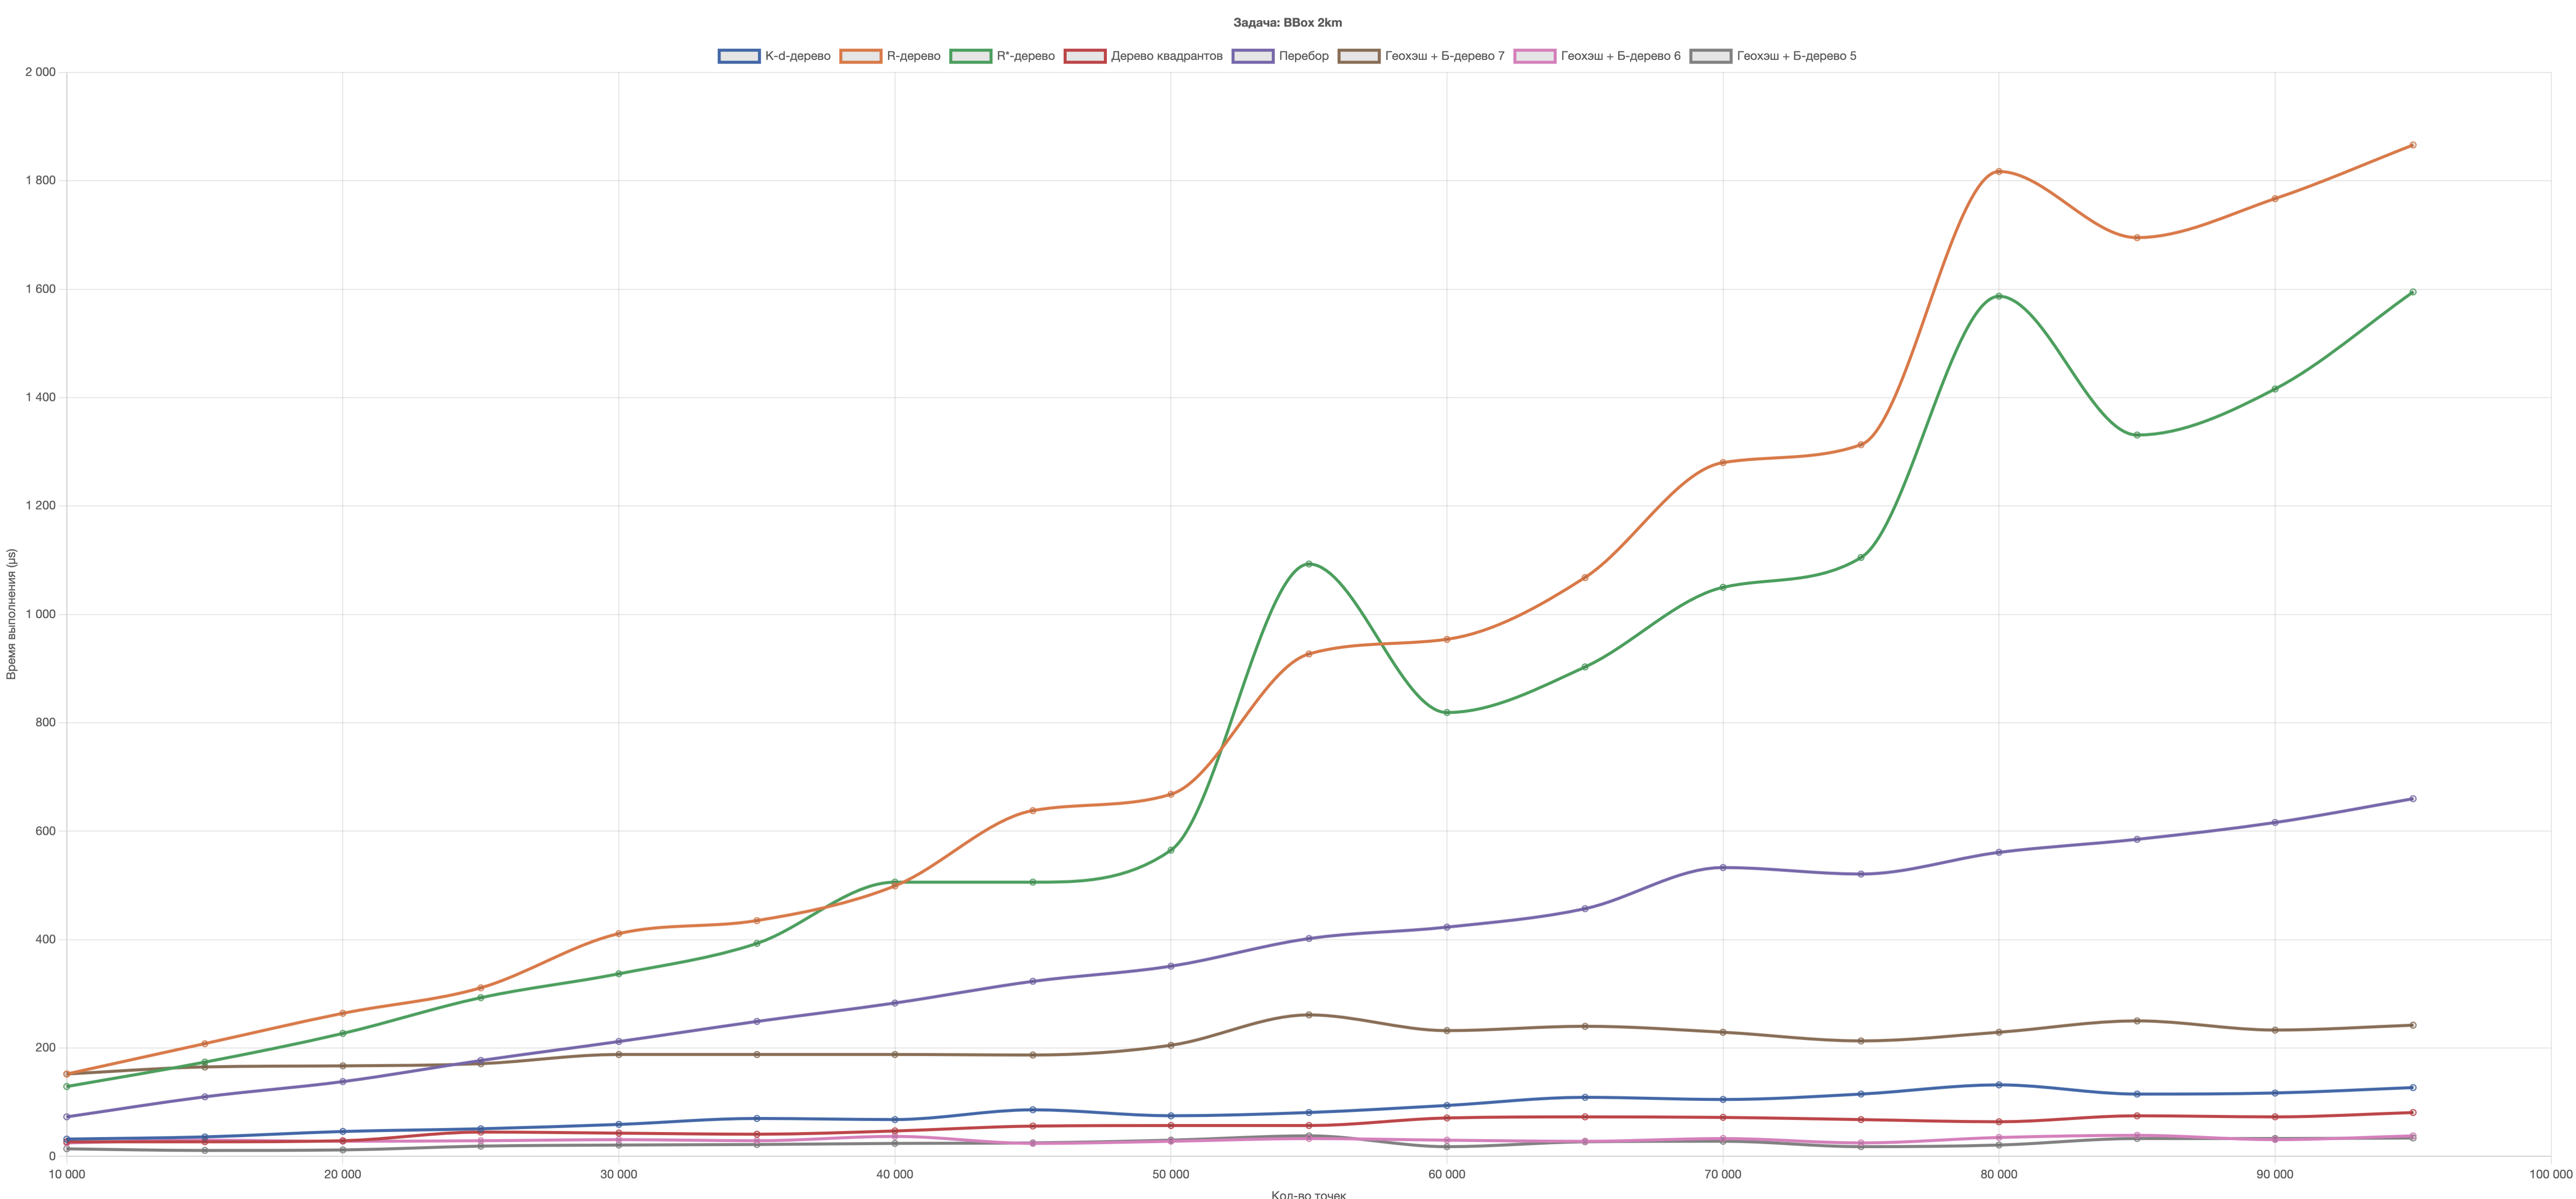
\includegraphics[scale=0.17]{results_app_1.png}
    \caption{Задача BBox на квадрате с ребром 2км}
\end{figure}

\begin{figure}[h]
    \centering
    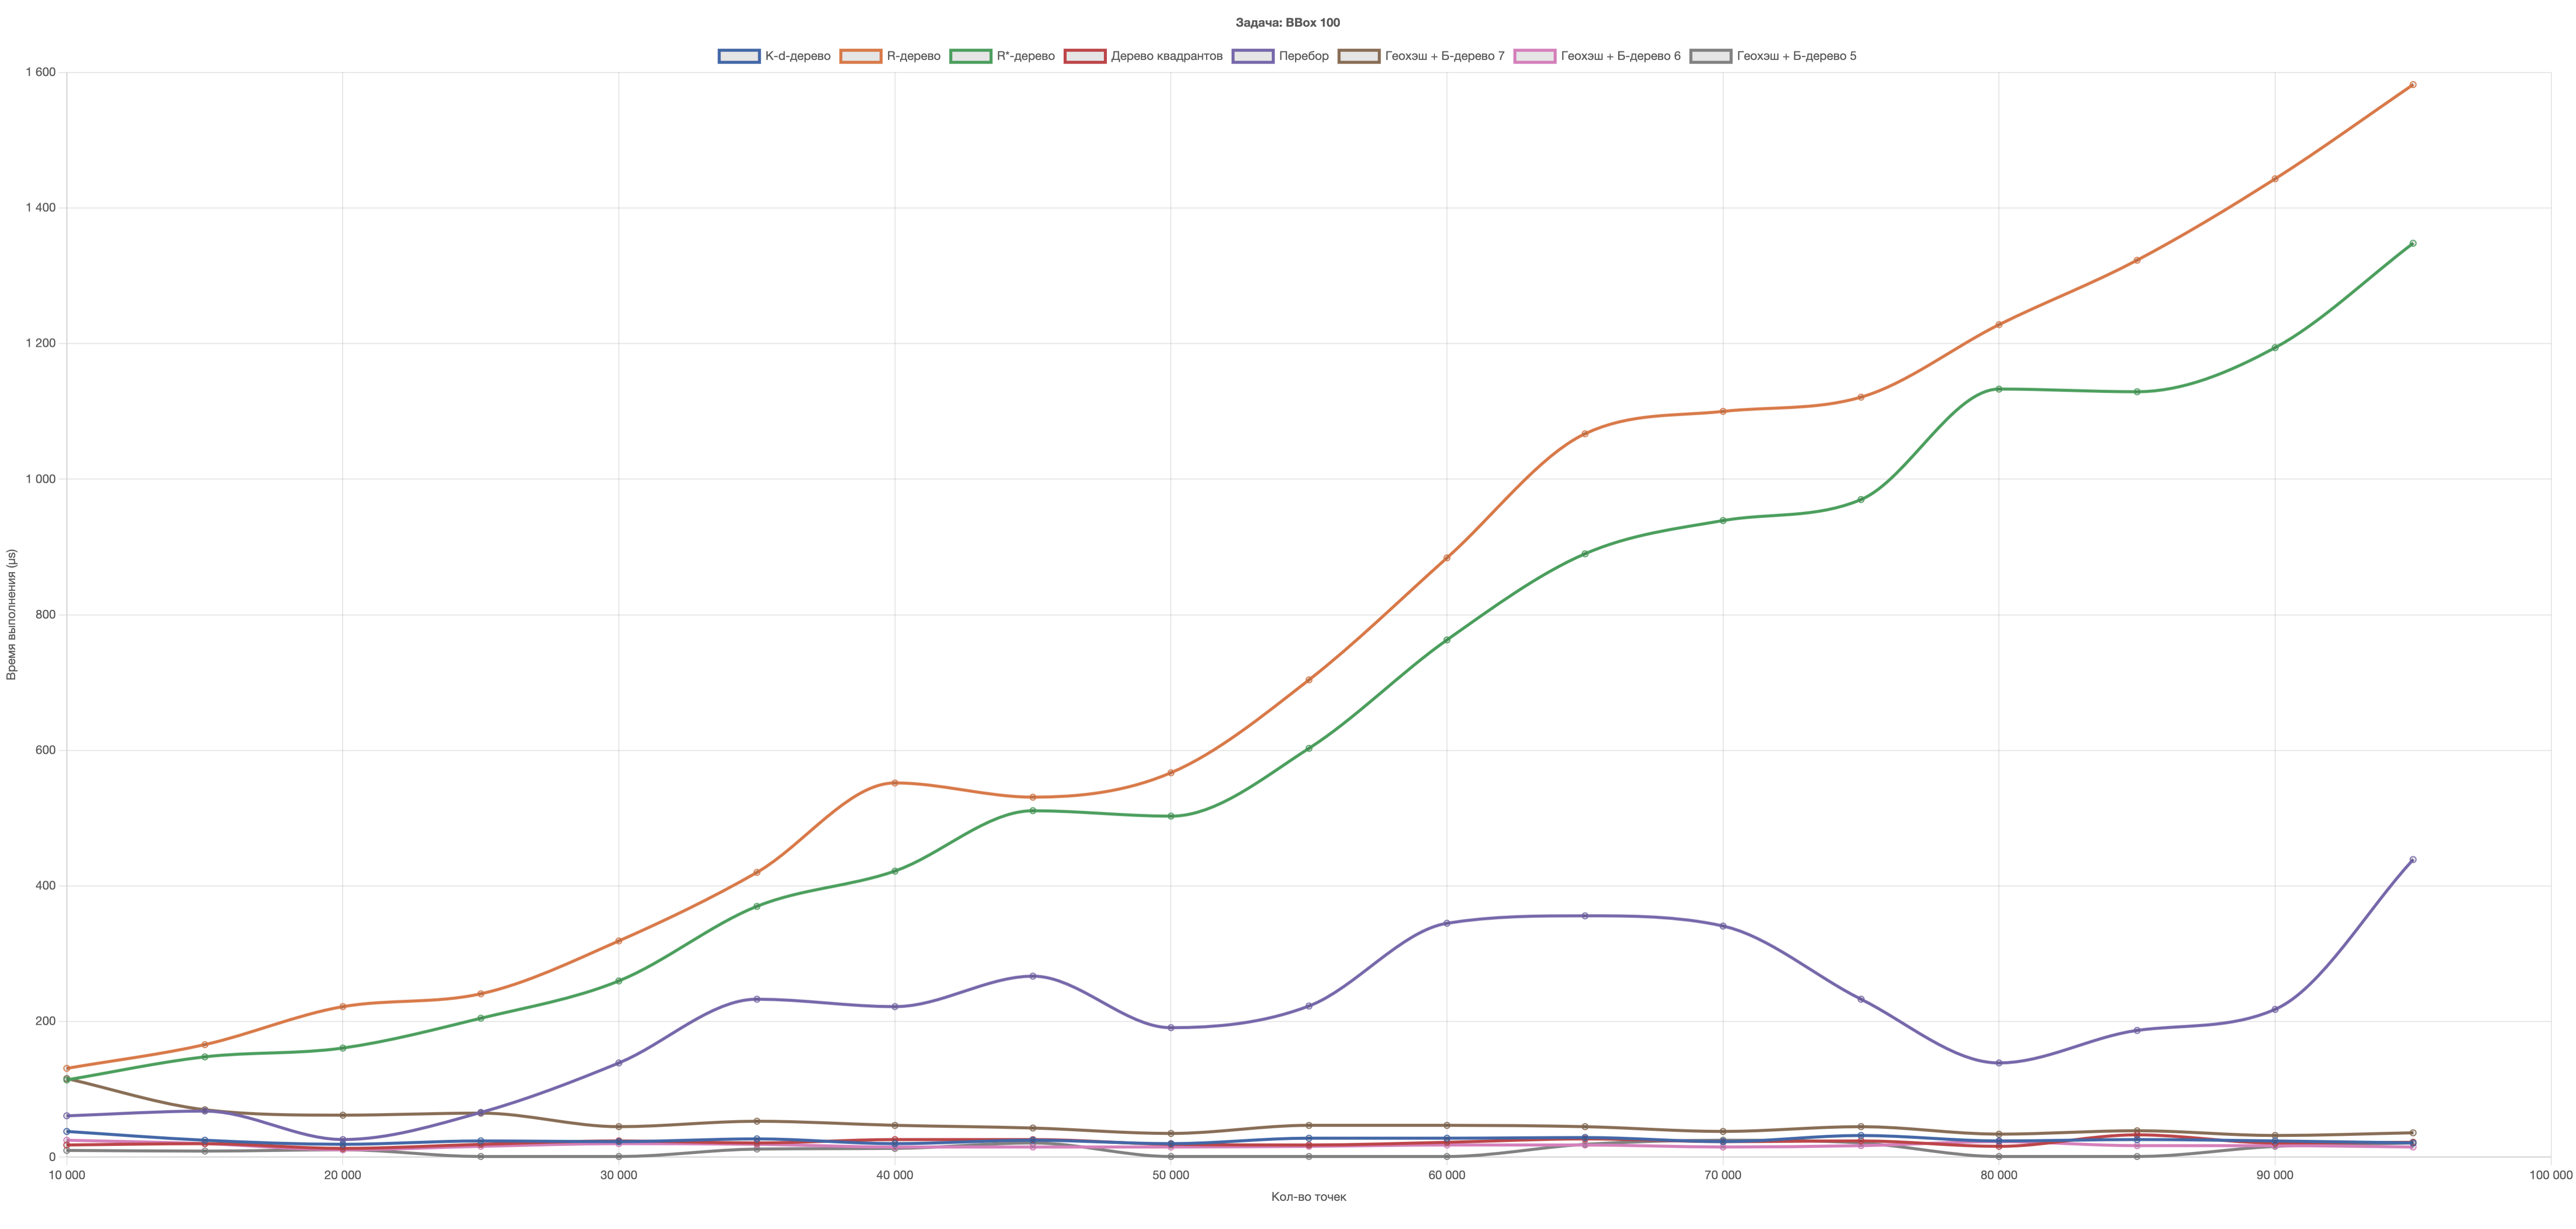
\includegraphics[scale=0.17]{results_app_2.png}
    \caption{Задача BBox на квадрате, в который входит не более 100 точек}
\end{figure}

\begin{figure}[h]
    \centering
    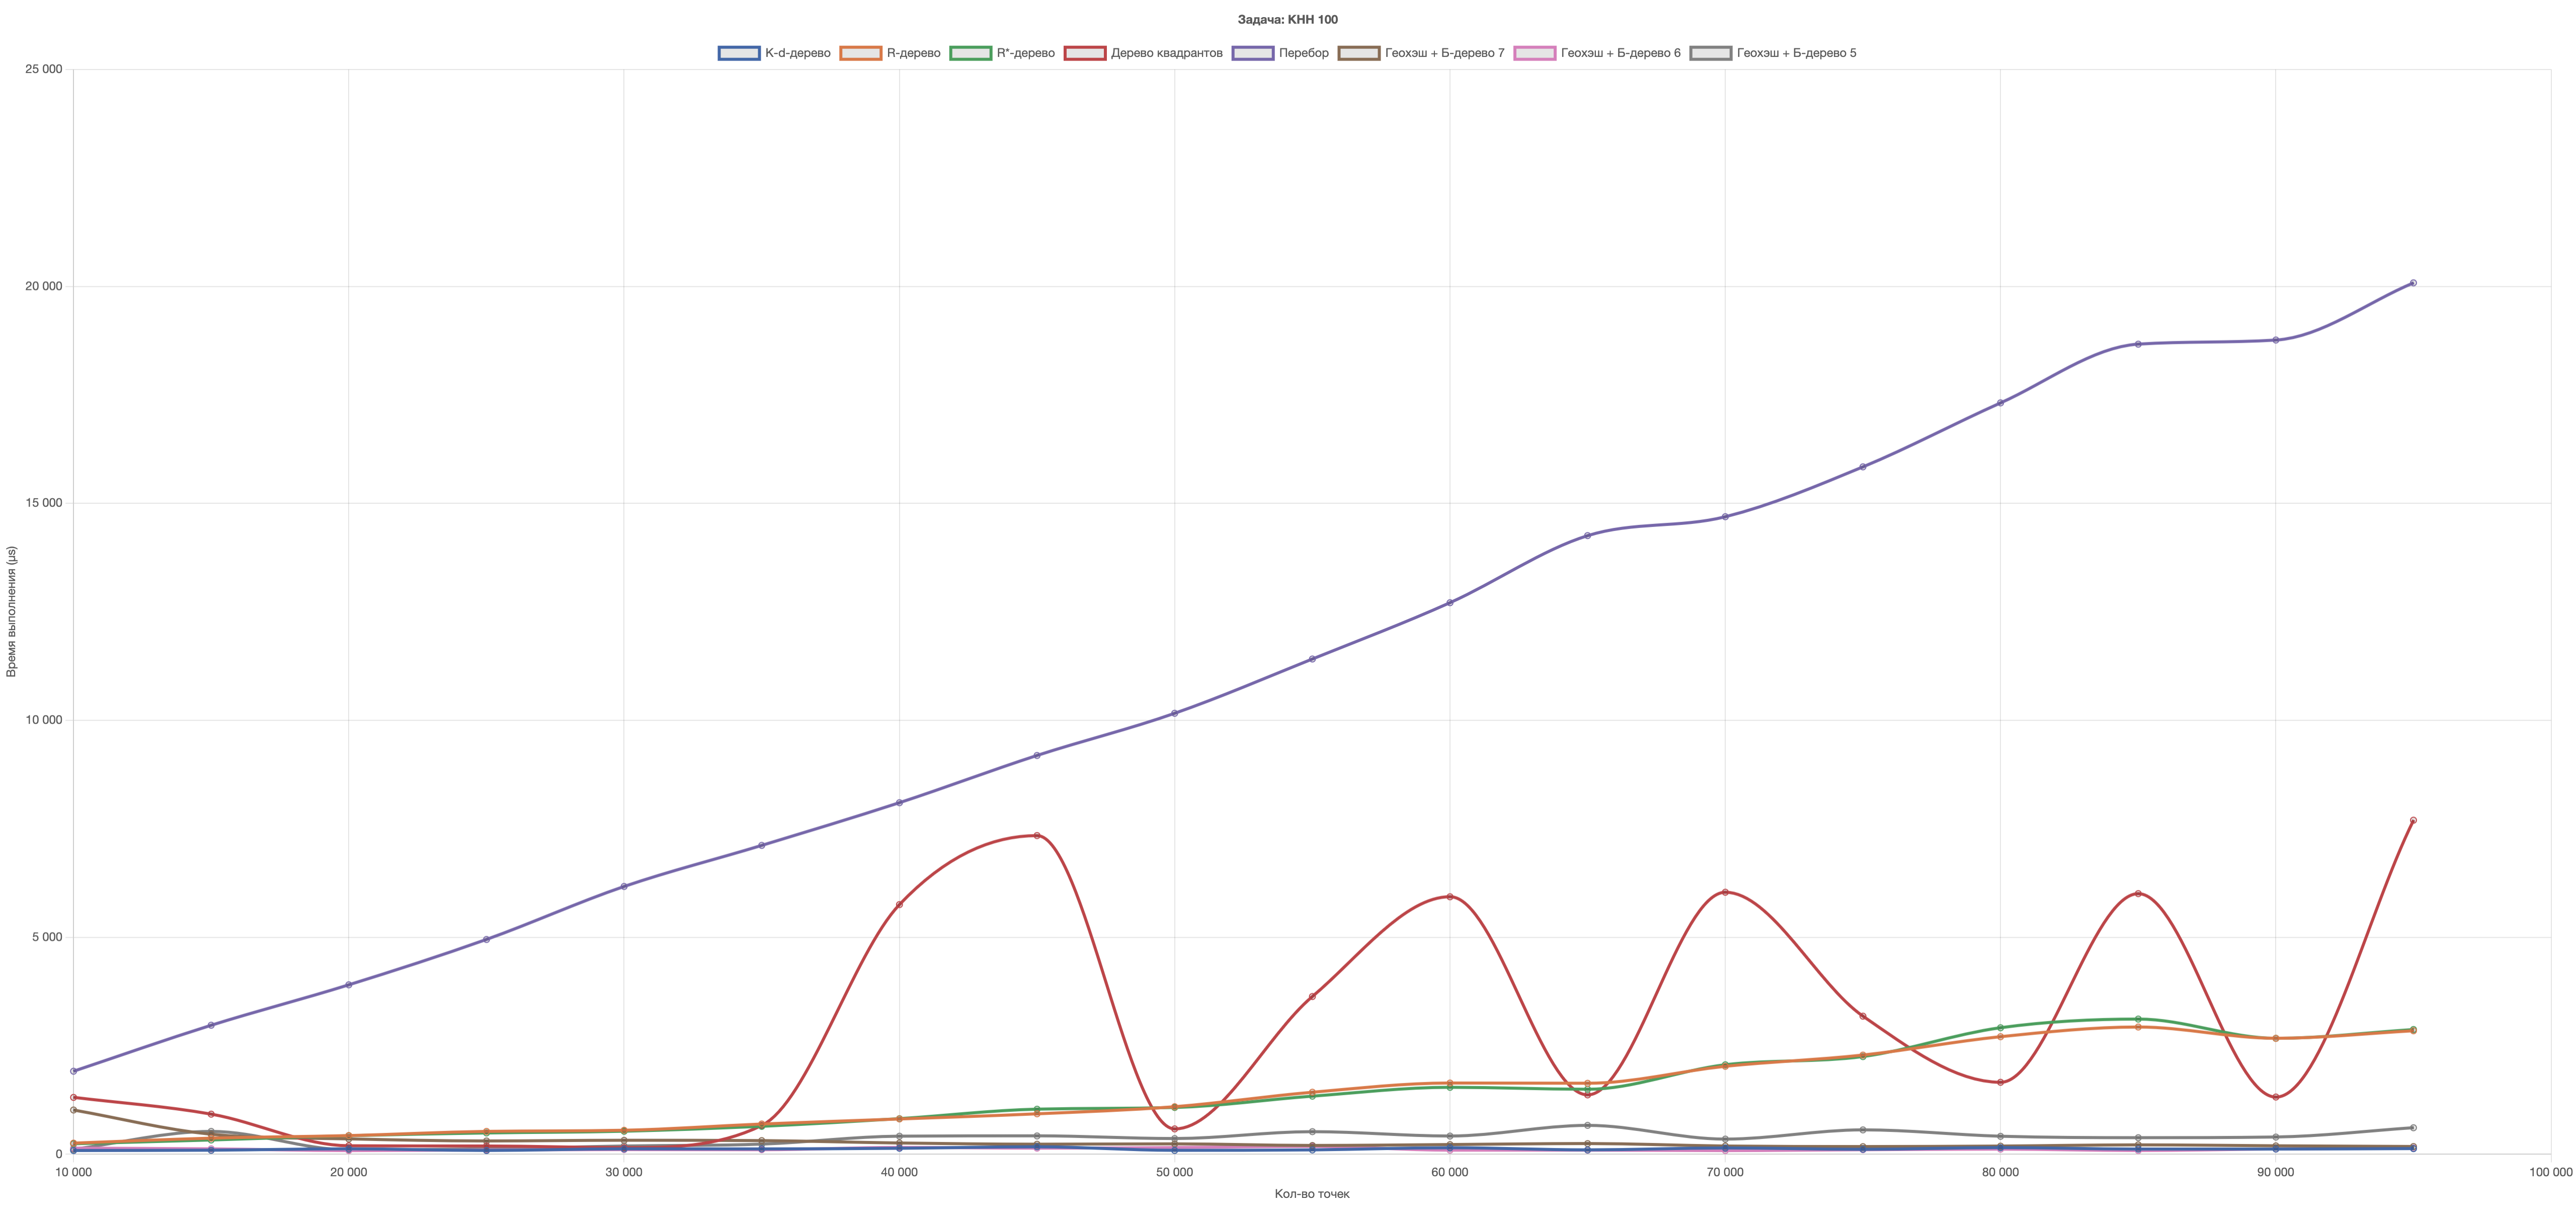
\includegraphics[scale=0.17]{results_app_3.png}
    \caption{Задача KNN на 100 точек}
\end{figure}

\begin{figure}[h]
    \centering
    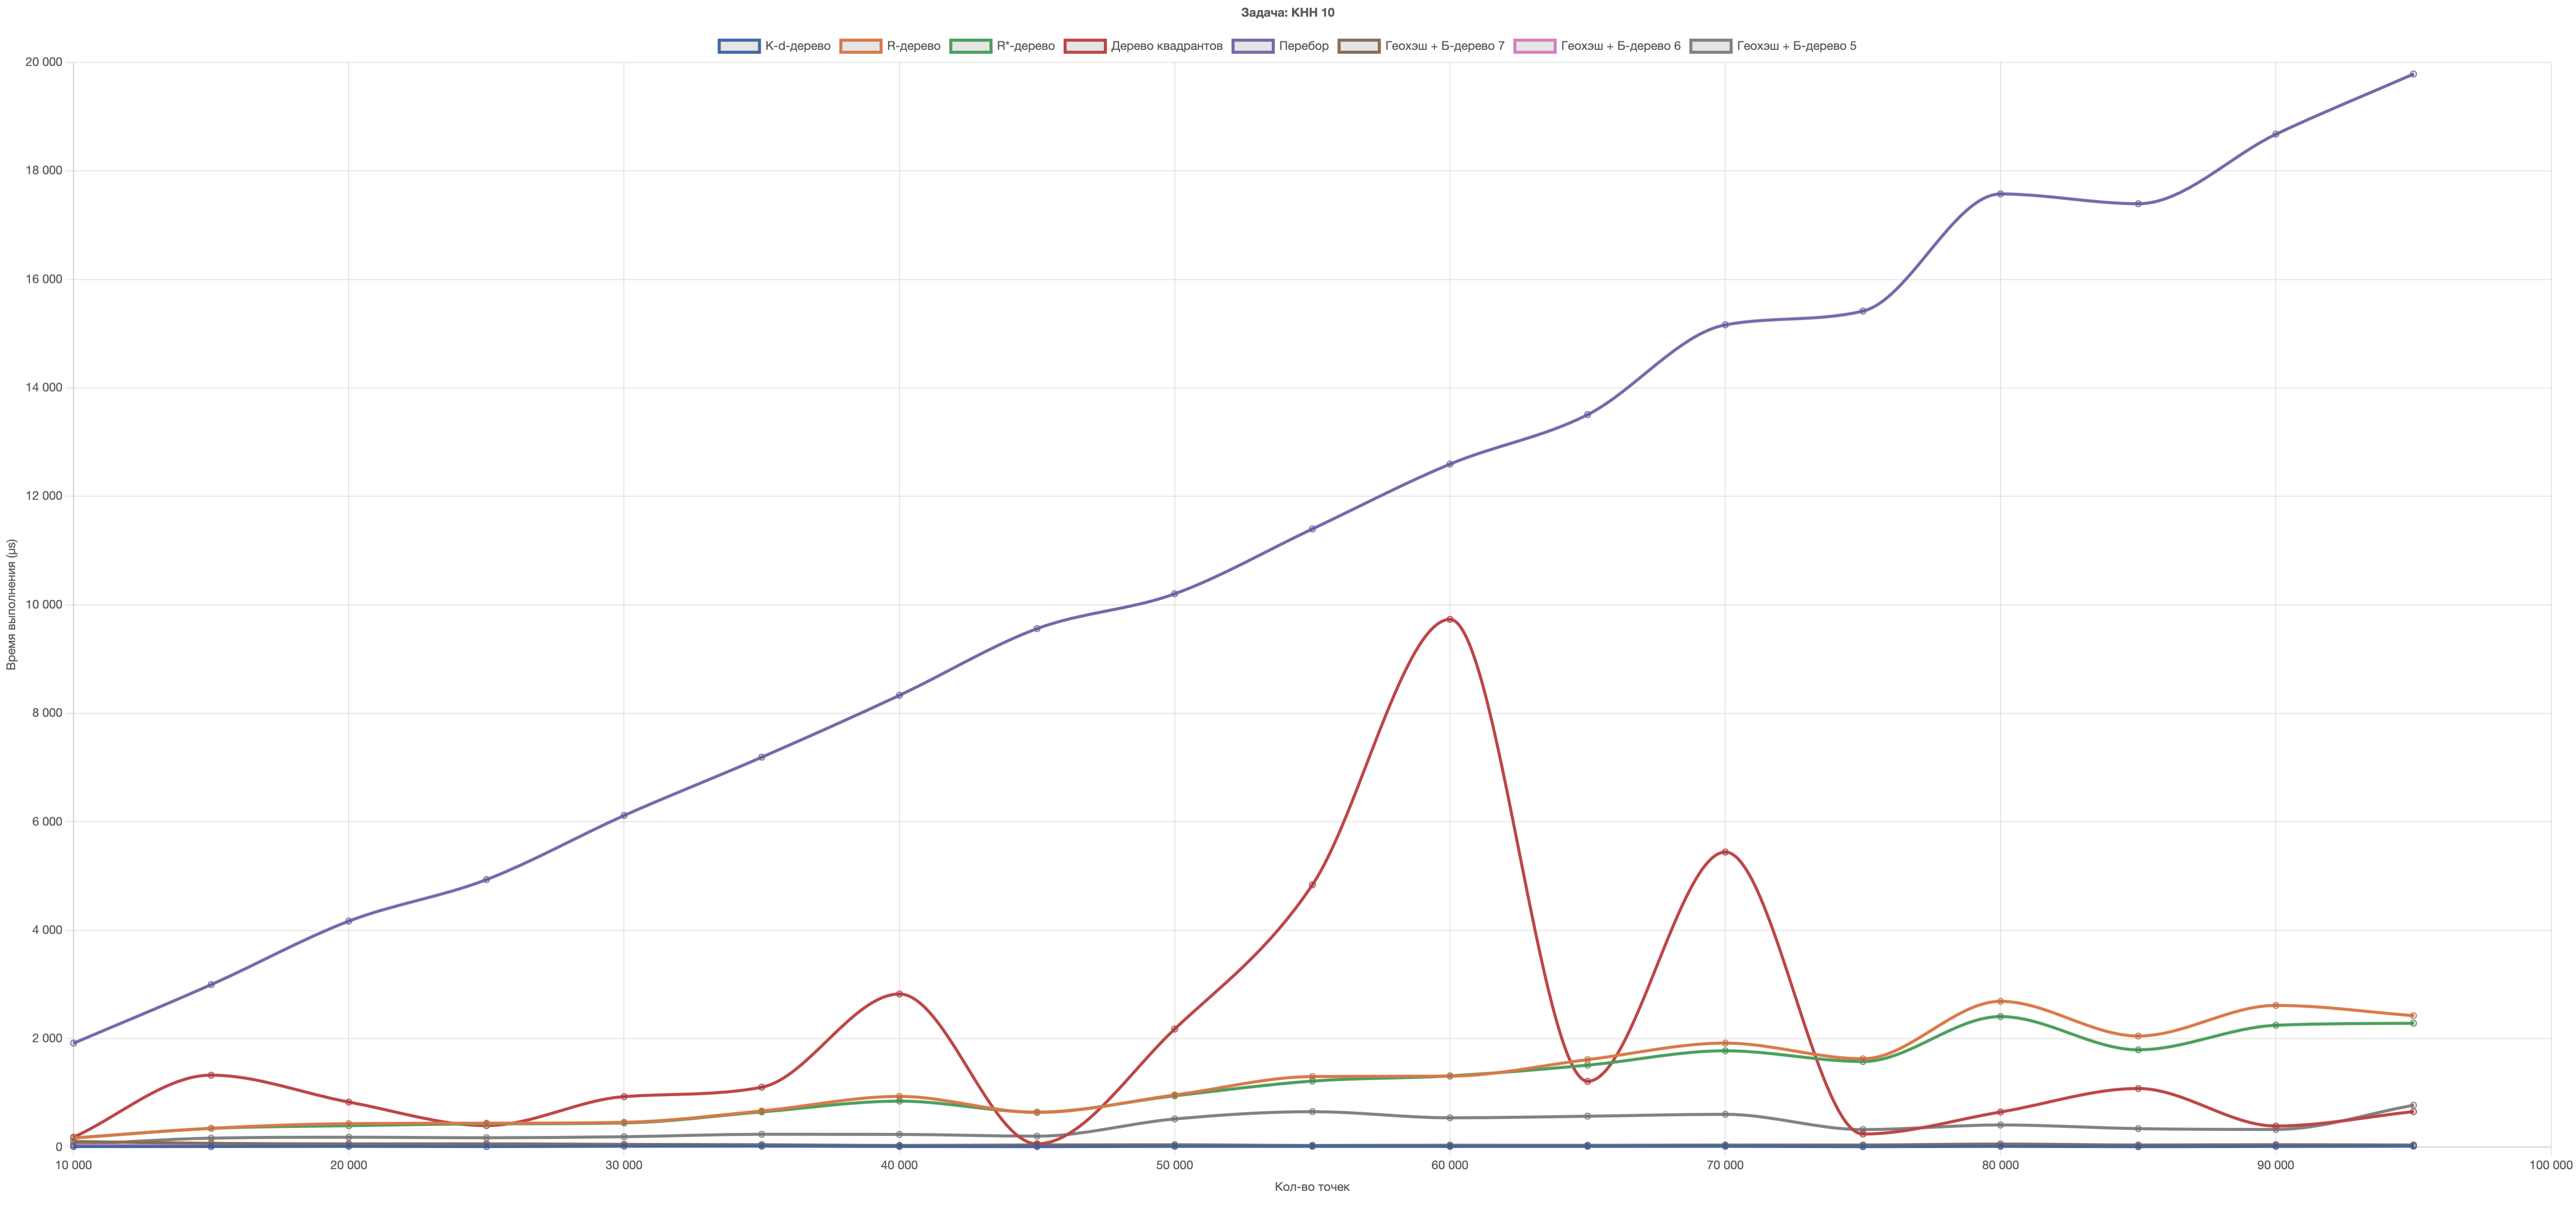
\includegraphics[scale=0.17]{results_app_4.png}
    \caption{Задача KNN на 10 точек}
\end{figure}

\begin{figure}[h]
    \centering
    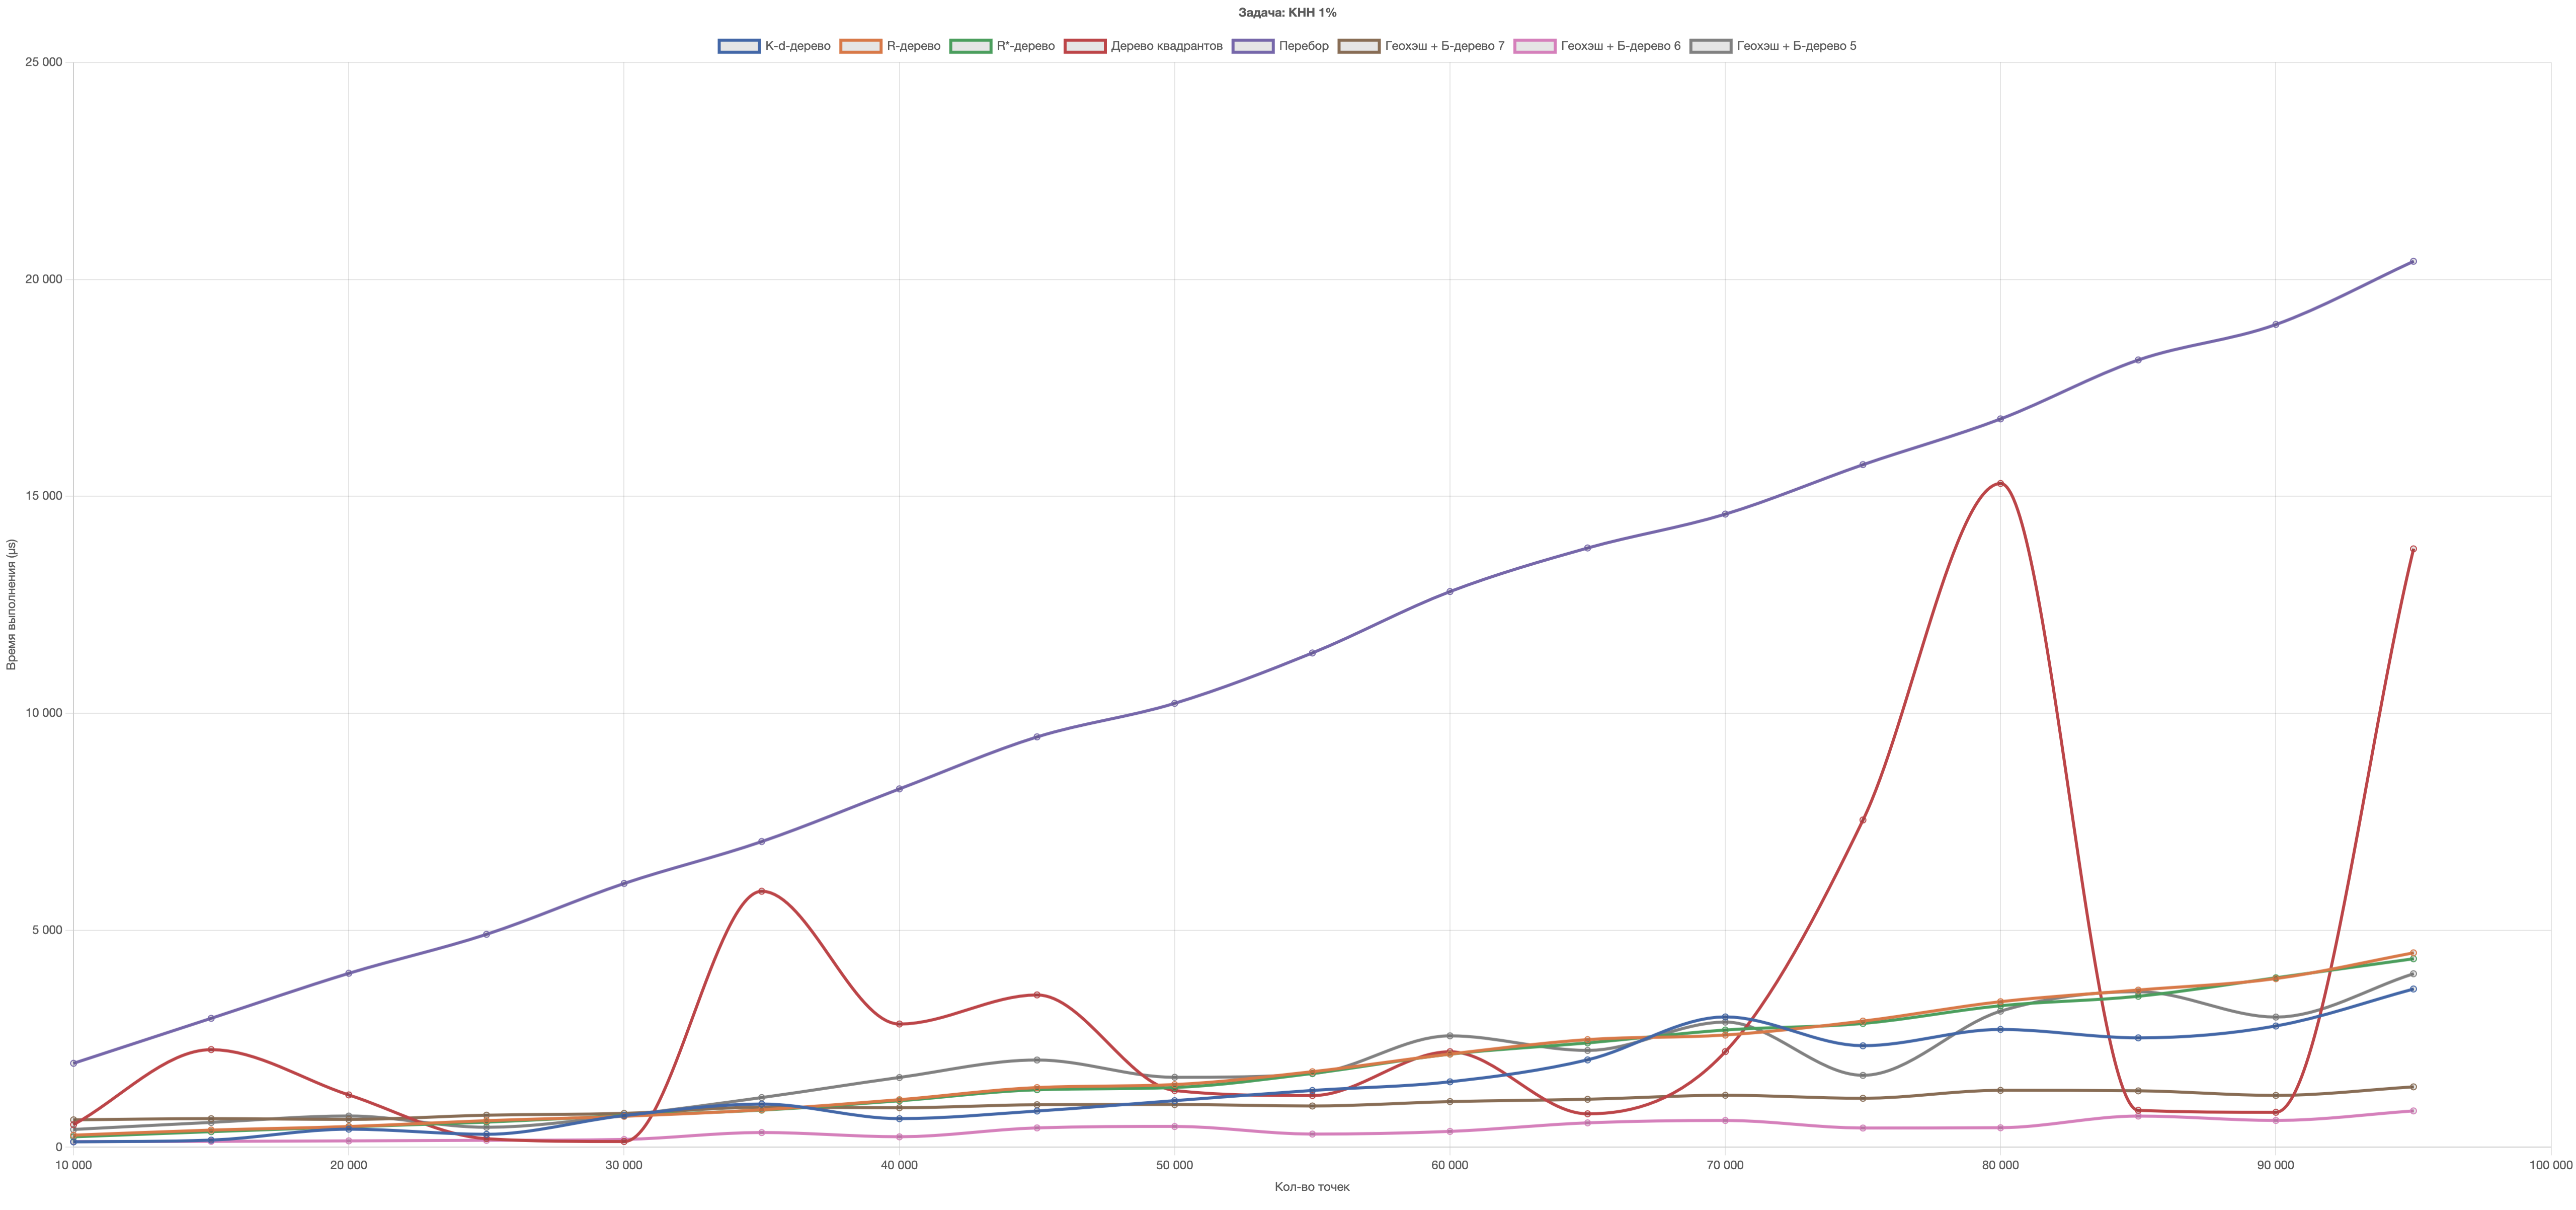
\includegraphics[scale=0.17]{results_app_5.png}
    \caption{Задача KNN на 1\% точек}
\end{figure}

\begin{figure}[h]
    \centering
    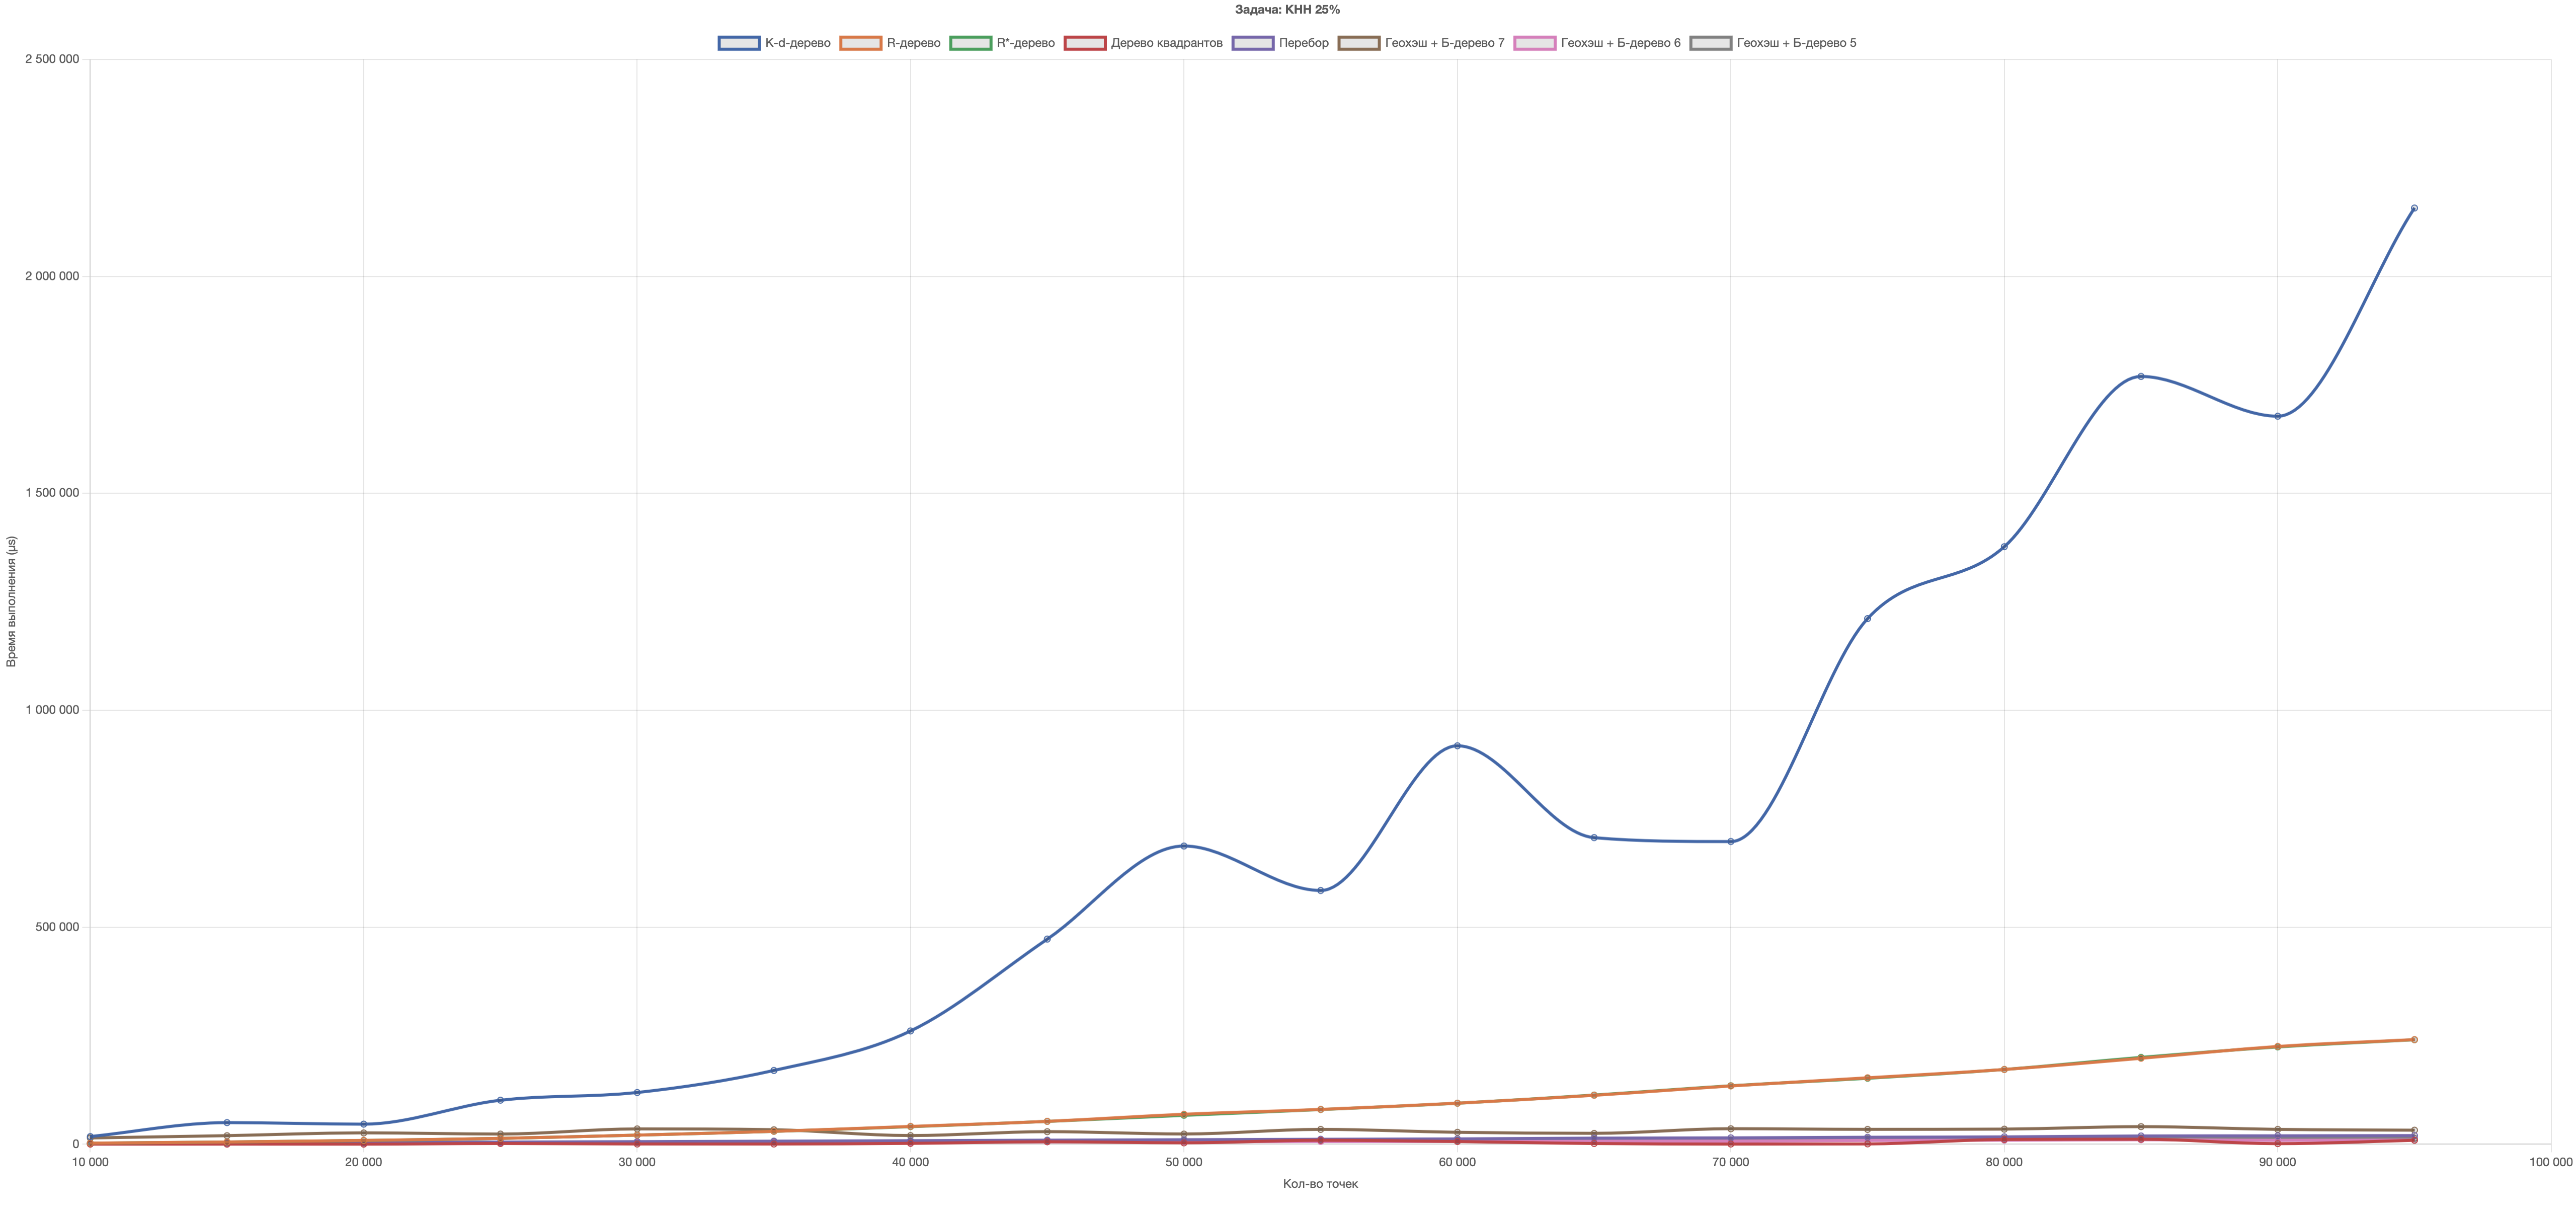
\includegraphics[scale=0.17]{results_app_7.png}
    \caption{Задача KNN на 25\% точек}
\end{figure}
я
\begin{figure}[h]
    \centering
    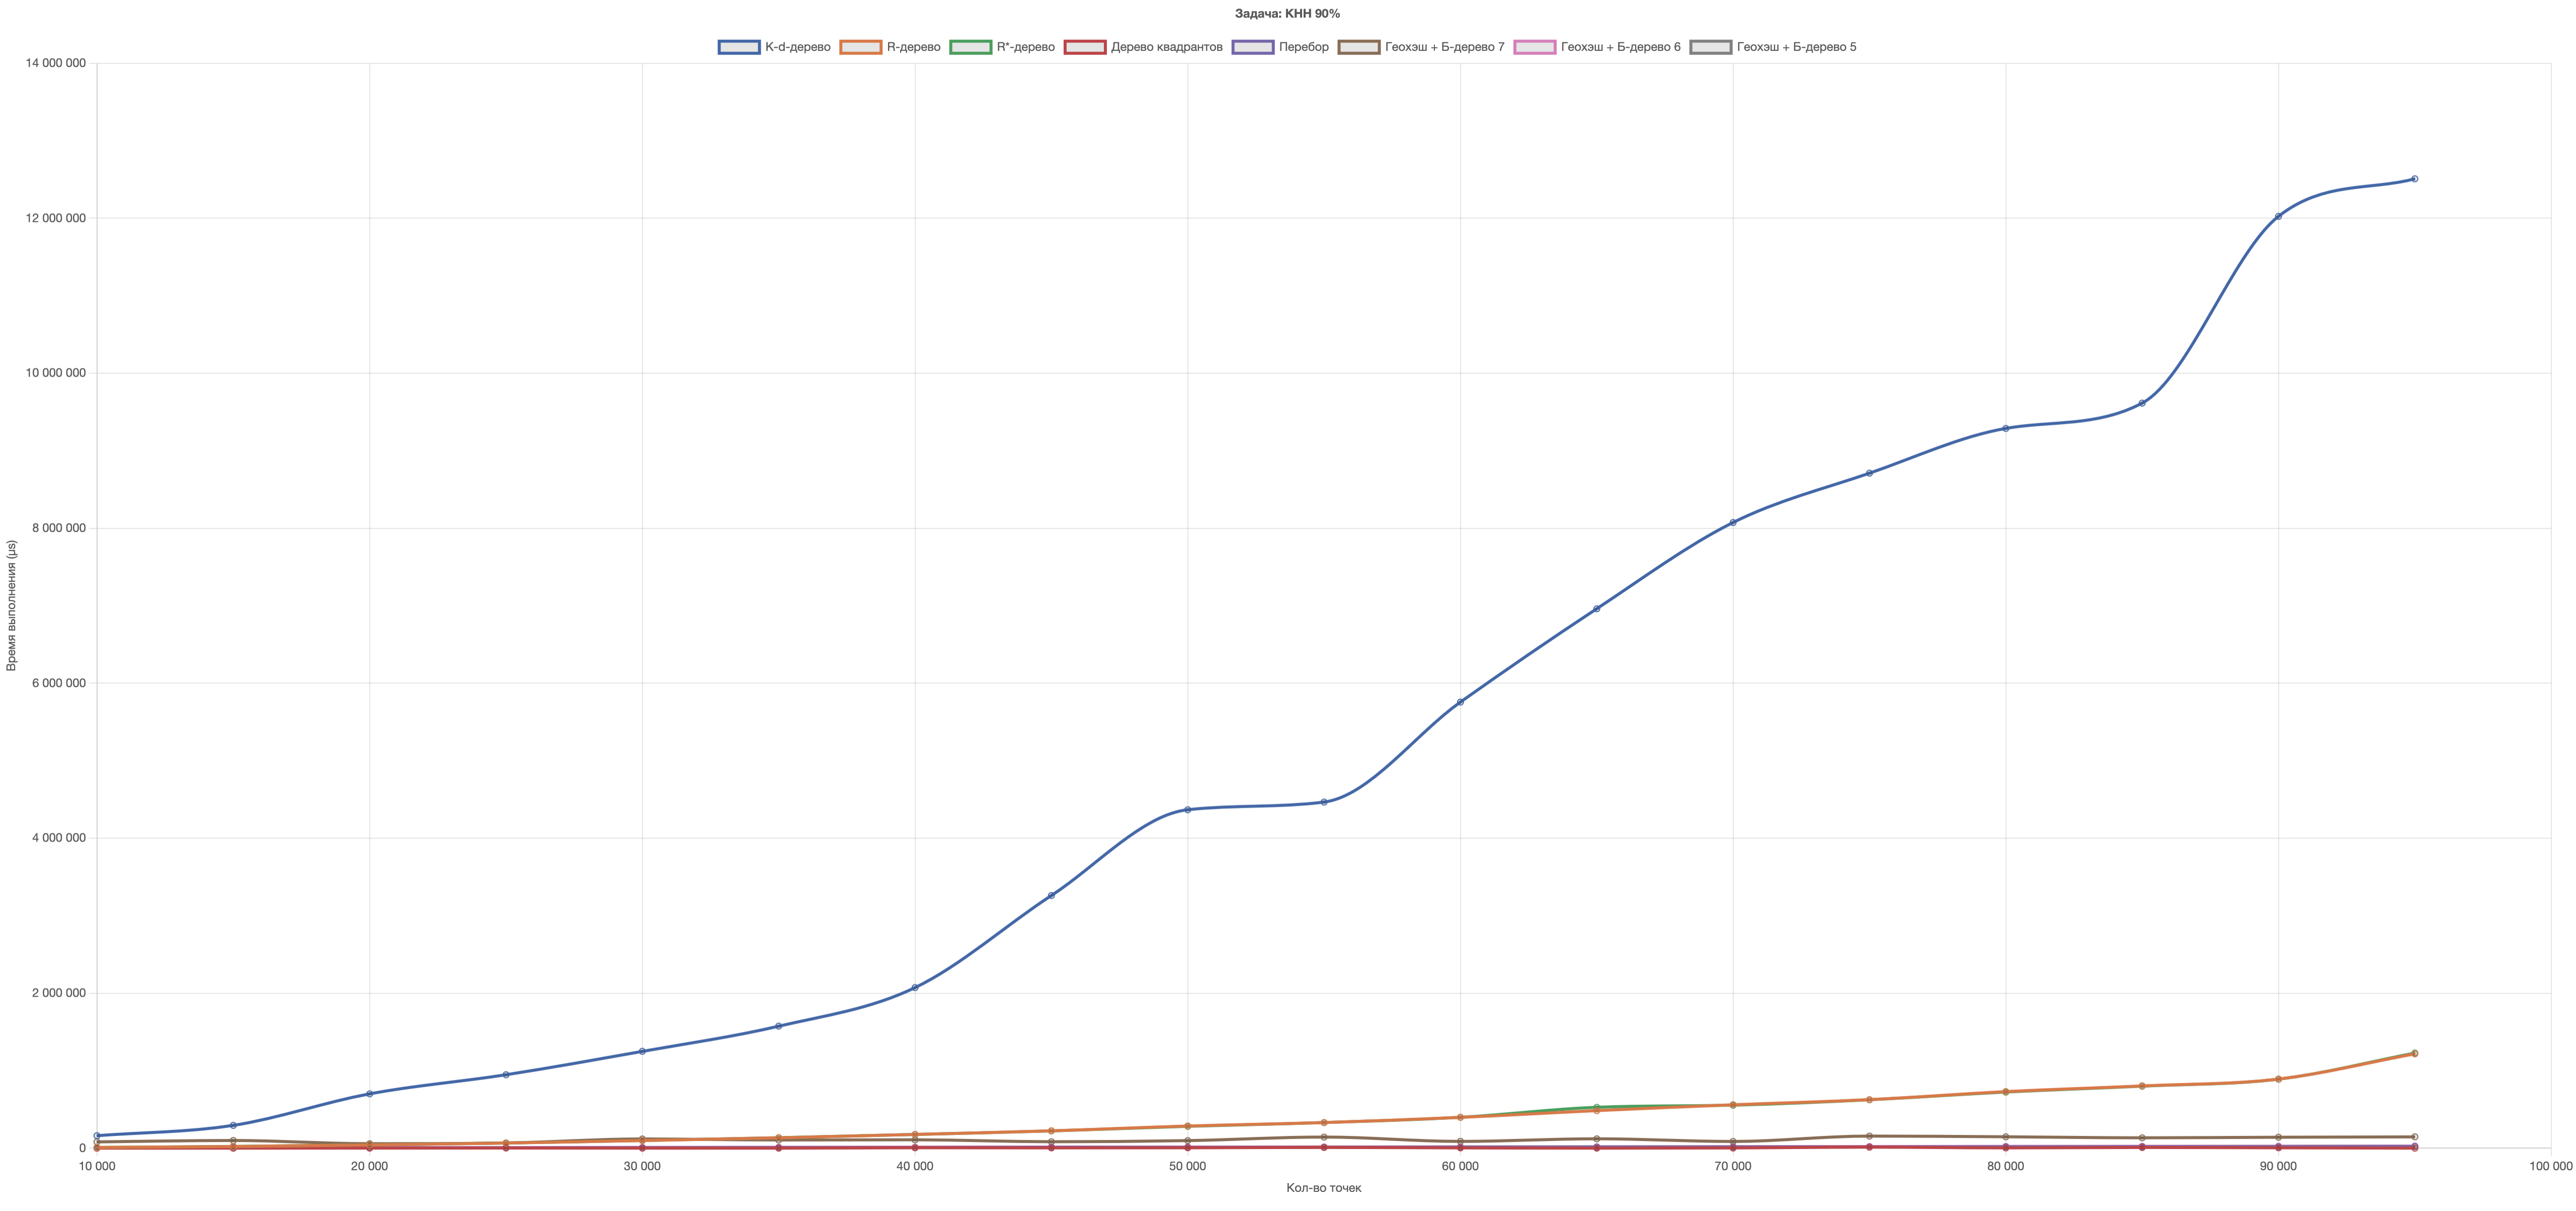
\includegraphics[scale=0.17]{results_app_6.png}
    \caption{Задача KNN на 90\% точек}
\end{figure}


